\chapter[Introduction]{Introduction}

\epigraph{I was born not knowing and have had only a little time to change that here and there.}
{\textit{Richard Feynman \\ Letter to Armando Garcia J.}}


\minitoc

\section{Motivation and context}

This work aims at exploring the port-Hamiltonian (pH) framework as a modelling paradigm, with particular emphasis for the case of flexible structures. This framework enjoys many interesting properties, since it intrinsically merges geometry with network and control theory \cite{vanderschaft2006book}. A powerful feature of this formalism, especially for the modelling task, is its modularity. Finite-dimensional port-Hamiltonian systems (pHs) can be easily interconnected together \cite{cervera2007interconnection}. The interconnection is also possible in the infinite-dimensional case \cite{kurula2010,augner2020int}. Eventually, it is also possible to merge finite and infinite pH systems \cite{pasumarthy2006}. This features is especially useful to simplify the modelling task in preliminary analyses, or, conversely, to achieve high-fidelity models of complex multiphysics phenomena. Examples of multiphysics problems are brain edema simulations \cite{ju2020brain} (cf. Fig. \ref{fig:p_brain}) or plasma physics \cite{nattila2019runko} (cf. Fig. \ref{fig:plasma}). \\



\begin{figure}[htbp]%
	\centering
	\subfloat[][Normal brain]{%
		\label{fig:p_normal}%
		\includegraphics[width=0.48\columnwidth]{part_1/brain_normal_p.eps}} 
	\hspace{8pt}%
	\subfloat[][Injured brain]{%
		\label{fig:p_injured}%
		\includegraphics[width=0.48\columnwidth]{part_1/brain_injured_p.eps}}%
	\caption[]{Simulated pressure within the brain for a physiological (left) and injured (right) condition. The authors propose a coupled multiphysics framework to solve the underlying Biot system. The numerical model is obtained using a combination of classical and mixed finite elements (courtesy of Mingchao Cai \cite{ju2020brain}).}%
	\label{fig:p_brain}%
\end{figure}

\begin{figure}[htbp]%
	\centering
	\subfloat[][Plasma density]{%
		\label{fig:rho_plasma}%
		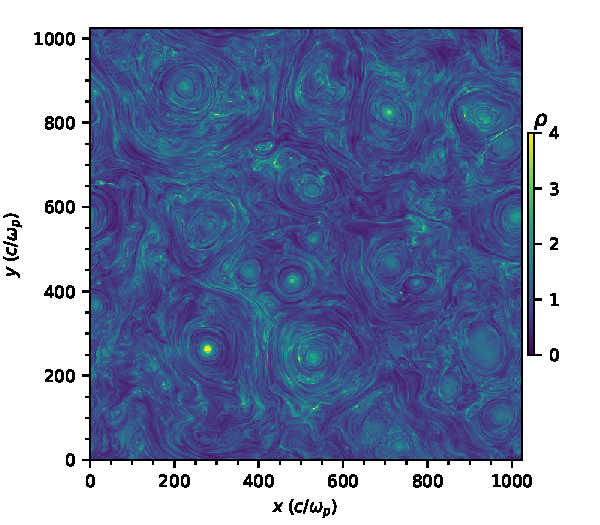
\includegraphics[width=0.48\columnwidth]{part_1/rho.pdf}}%
	\hspace{8pt}%
	\subfloat[][Out-of-plane plasma current density]{%
		\label{fig:jz_plasma}%
		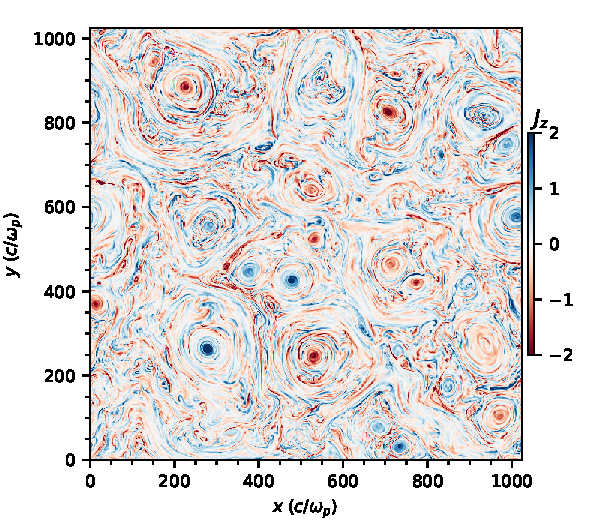
\includegraphics[width=0.48\columnwidth]{part_1/jz.pdf}} 
	\caption[]{Simulated snapshot of the density field (left) and current density (right) for plasma kinetic turbulence. The underlying code employs the Yee finite difference scheme \cite{yee1966numerical} to approximate the Vlasov-Maxwell equations and a full relativistic Boris scheme \cite{boris1970relativistic} to update the particles velocity and position (courtesy of Joonas N\"attil\"a \cite{nattila2019runko}).}%
	\label{fig:plasma}%
\end{figure}

The port-Hamiltonian framework has been extensively used to model and control distributed system arising from a variety of physical models: Timoshenko \cite{macchelli2004timo} and Euler-Bernoulli  \cite{aoues2017modeling} beam models, acoustic wave propagations \cite{trenchant2018}, stirred tank reactors \cite{ramirez2013irreversible},  plasma in tomahawks \cite{vu2016plasma} and fluid-structure interactions \cite{cardoso2017}. The large majority of these examples refer to 1-dimensional models. Indeed, for 1-dimensional linear PH systems with a generalized skew-adjoint system operator, \cite{legorrec2005} gives conditions on the assignment of boundary inputs and outputs for the system operator to generate a contraction semigroup. This result has been largely used to construct passive boundary controllers for hyperbolic systems \cite{villegas2009exponential,macchelli2016synthesis,macchelli2020exponential}. \\

Since their introduction, distributed port-Hamiltonian systems (dpHs) have been defined on multidimensional spatial domains using the language of differential forms \cite{vanderschaft2002}. In \cite{villegas2007} pH  modelling and semigroup approach of infinite-dimensional systems are merged together. Therein, the  case of multidimensional domains is only briefly discussed. Many other examples of pHs on multidimensional domains are detailed in \cite[Chapter 4]{duindam2009}. However, well-posedness results are not presented there. A first contribution in this sense can be found in \cite{zwart2015wave}, where the authors demonstrate the well-posedness of the linear wave equation in arbitrary geometric dimensions. The recent paper  \cite{skrepek2019wellposedness} generalizes this result to treat the case of generic first order linear pHs in arbitrary geometric dimensions. Despite all this preexisting literature, models arising from structural mechanics on multidimensional domains have almost never been considered (apart from the notable exception of \cite{macchelli2005mindlin}).  \\

The potential of the pH framework as modelling paradigm has been recently explored by researchers. For instance, in \cite{egger2018damped} the authors consider a port-Hamiltonian model for pressure waves propagation in networks of pipes. By employing a mixed finite element scheme, the authors achieve a structure-preserving discretization of the original model. A model reduction algorithm for this discretized model of pipeline network is then discussed in \cite{egger2018}. These recent works substantiate the validity of this framework to tackle complex application scenarios and highlight the importance of structure-preserving discretization algorithms. Disposing of methodologies capable of constructing reliable discretizations is important not only for simulation, but also for control purposes. In particular in \cite{toledo2020} the authors develop a systematic synthesis method for observer-based boundary controller design for pHs on one dimensional spatial domains. To construct the observer, a suitable discretized version of the system is assumed to be available. \\

This thesis tries to establish a clear connection between linear structural mechanics models and port-Hamiltonian systems, both for the modelling and discretization task. These two tasks are indeed strongly related in the context of pHs. To get a pH formulation for elasticity models, one has to introduce the stress variable, associated to the deformation energy, as a additional principal unknown. Adding the stress variable as an unknown is the starting point of mixed finite elements \cite{arnold1990intro}. This leads to the decomposition of the initial elliptic operator (i.e. the Laplacian or bi-Laplacian), into two formal adjoint operators. By consequence, the dynamics is regulated by a formally skew adjoint operator, hence leading to an Hamiltonian system. After performing an integration by parts, a mixed discretization is immediately achieved \cite{joly2003variational}. This very concise reasoning informally elucidates the strong connection between port-Hamiltonian modelling of continuum mechanics and mixed finite elements. 


\section{Literature review}
A brief literature review of the topics considered in the thesis is made here. Throughout the chapters of the thesis, the literature is also referenced.


\subsection{Structure-preserving discretization}

The research community is focusing on structure-preserving discretization techniques since several years. The first study dates back to \cite{golo2004hamiltonian}, where the authors made use of a mixed finite element spatial discretization for 1D and 2D hyperbolic system of conservation laws. Pseudo-spectral methods relying on higher-order global polynomial approximations were studied in \cite{moulla2012pseudo}. This method was used and extended to take into account unbounded control operators in \cite{cardoso2017}. A simplicial discretization based on discrete exterior calculus was proposed in \cite{seslija2012discrete}. This approach comes with additional complexities, since a primal and a dual meshes have to be defined but the discretization is structure-preserving, regardless of the spatial dimension of the problem. Weak formulations which lead to Galerkin numerical approximations began to be explored in the last years. In \cite{kotyczka2018weak} the prototypical example of hyperbolic systems of two conservation law was discretized by a weak formulation. In this approach the boundary is split according to the causality of boundary ports, so that mixed boundary conditions are easily handled. The construction of the necessary power-preserving mappings is, however, not straightforward on arbitrary meshes. A 2D finite difference method with staggered grids was used in \cite{trenchant2018}.

\subsection{Mixed finite elements for elasticity}

Thanks to \cite{cardoso2018pfem}, it has become evident that there is a strict link between  discretization of port-Hamiltonian (pH) systems and mixed finite elements. Velocity-stress formulation for the wave dynamics and elastodynamics problems are indeed Hamiltonian and their mixed discretization preserves such a structure. For instance in \cite{kirby2015} the authors employed mixed finite elements to obtain a  symplectic semi-discretization for the wave equation. This allows using known finite element scheme to preserve the pH structure at the discrete level. \\

This discretization technique is a mature research topic, that is rather advantageous over classical finite elements, for a variety of reasons \cite{wriggers2009}:
\begin{itemize}
	\item locking-free behavior for incompressible material,
	\item no locking in thin elements,
	\item no sensitivity against mesh distortions,
	\item good coarse mesh accuracy, 
	\item simple implementation of non-linear constitutive equations and
	\item efficiency (e.g. few necessary integration points).
\end{itemize}

Mixed finite elements for the wave equation have been studied in \cite{geveci1988,becache2000wave}. For elastodynamics the construction of stable elements gets more complicated because of the presence of the symmetric stress tensor. Existing elements enforce symmetry either strongly \cite{becache2001elas,arnold2002mixed} or weakly \cite{arnold2007mixed,arnold2014elastodynamics}. A complete comparative study on this topic can be found in \cite{lee2012mixed}. \\

For what concerns the mixed discretization of Kirchhoff like plate, non-conforming elements are the most common solution to lower the regularity requirement for this problem \cite{arnold1990intro}. In particular the Hellan-Herrmann-Johnson method \cite{hellan1967,herrmann1967finite,johnson1973convergence} is the most successful one. Generic boundary conditions are not easy to handle. Nevertheless, the method is convergent for all usual boundary conditions \cite{blum1990}. Recently a mixed discretization requiring $C^0$ elements and valid for all kind of boundary condition has been proposed in \cite{rafetseder2018siam} for static bending problems. However, this method requires the resolution of three consecutive to solve problems, hence the extension to the dynamical case is not straightforward. \\

There are many more important papers on this topic. Those cited here are significant since many proposed discretizations are based on them.

 
\subsection{Modular multibody dynamics modelling}

In structural control co-design of flexible multibody systems, it is especially useful to dispose of a modular description, to simplify analysis. In this spirit, the transfer matrix method \cite{rong2010transfer} and the component mode synthesis \cite{hurty1965cms} are two well known substructuring techniques that allow the construction of complex multibody systems by interconnecting subcomponents together. A reformulation of the Finite Element-Transfer Matrix (FE-TM) method \cite{tan1990transfer} allows an easy construction of reduced models that are suited for decentralized control design. For the component mode synthesis, the controlled component synthesis (CCS), a framework for the design of decentralized controller of flexible structures, has been proposed in \cite{young1990}. Another modeling paradigm based on the component mode synthesis is the two-input two-output port (TITOP) approach \cite{alazard2015titop}. It conceives the dynamical model of each substructure as a transfer between the accelerations and the external forces at the connection points. This feature allows considering different boundary conditions by inverting specific channels in the transfer matrix. A rigorous validation was provided in \cite{perez2016flexible,sanfedino2018finite}, where the robustness of the methodology in handling various boundary conditions was assessed. \\

The Lagrangian formulation is the most commonly used methodology to retrieve the equations of motion of flexible multibody systems. The strong form Lagrangian formulation of flexible dynamics using a floating frame approach is detailed in  \cite[Eq. 4.10]{simeon2013computational} using the least action principle, but without highlighting the Hamiltonian structure of the problem.  Using the variational principles of geometric mechanics the equations of motion in Hamiltonian form can be derived either for rigid body dynamics \cite[Proposition 7.1.1]{holm2008geometric} and general non linear elasticity \cite[Chapter 3]{marsden1981lectures}. The port-Hamiltonian (pH) framework \cite{duindam2009} has been recently employed to describe the dynamics of rigid and flexible links \cite{macchelli2007link,macchelli2009multi}. Being intrinsically modular, the pH approach naturally allows constructing complex system by interconnecting together atomic elements. The formulation therein naturally accounts for the non-linearities due to large deformations.  However, this methodology relies on Lie algebra and differential geometry concepts and requires non standard discretization techniques. Thus, the overall implementation is not straightforward. \\

\indent Together with the approach used to derive the equations of motion, the incorporation of the elastic motion represents another important point when dealing with flexible multibody systems. Three descriptions are commonly used: the floating frame formulation, the corotational frame formulation and the inertial frame formulation \cite{ellenbroek2018}. The choice greatly depends on the foreseen application.  The corotational and inertial frame formulations take into account large deformations of the elastic body, hence are well-suited for accurate simulations. For these formulation many model reduction strategies have been developed in the last two decades \cite{rong2019}. The inclusion of active control strategies is often unfeasible due to the computational burden \cite{wasfy2003survey}. The floating frame formulation is less accurate but easily integrates many model reduction techniques \cite{nowakowski2012}, making it possible to obtain a low-dimensional problem for control design. \\


\section{Outline}

The flowchart of thesis is illustrated in Fig. \ref{fig:flowchart}. The thesis in divided into four main parts.

\paragraph{Part I (Chapters 1, 2)}
This part gives a general introduction of the following work. Chapter \ref{ch:reminder} briefly remind what  finite- or infinite- dimensional pH systems are and how these systems are deeply related to the geometric Dirac  or Stokes-Dirac structure (for the finite- and infinite- dimensional case respectively).

\paragraph{Part II (Chapters 3, 4, 5)}
This part is devoted to the formulation of suitable models for elasticity and thermoelasticity. This part is subdivided into three chapters.
\begin{itemize}
\item Chapter \ref{ch:elasPH} details the pH formulation for general n-D linear elasticity.
\item A pH formulation of thin (Kirchhoff-Love) and thick (Mindlin-Reissner) plate models is given in Chapter \ref{ch:platePH}.
\item The linear fully coupled thermoelastic problem is modelled as a coupled pH system in Chapter \ref{ch:Thermo}. 
\end{itemize}


\paragraph{Part III (Chapters 6, 7, 8)} This part is dedicated to the discussion and implementation of the main discretization tool: the Partitioned Finite Element method. This method is a natural extension to pHs of mixed finite elements. This part consists of three chapters.
\begin{itemize}
	\item A detailed description of the operating principle of PFEM is given in Chapter \ref{ch:pfem}. The approximation bases for this discretization are not explicitly defined in this chapter, since the method can be implemented through finite elements and spectral methods.
	\item A convergence study of several finite elements is illustrated in Chapter \ref{ch:conv} for the bending of thin structures (beams and plates). This is by no means a rigorous mathematical convergence analysis. However, thanks to preexisting results in the literature, error estimates are conjectured and validated through numerical experiments.
	\item Chapter \ref{ch:applications} is dedicated to the applications of the PFEM. In particular, the focus is on stabilization by damping injection, enforcement of mixed boundary conditions and validation of the thermoelastic pH model for an analytical solution.
\end{itemize}
 
\paragraph{Part IV (Chapters 9, 10)} In this part a pH formulation of flexible multibody systems is discussed an validated. Chapter \ref{ch:fmdPH} details the derivation of a pH system associated to a flexible floating body under small deformation assumption. Several tests are then performed in Chapter \ref{ch:valid}.


\begin{sidewaysfigure}
	\centering
	\includegraphics[width=0.95\columnwidth]{part_1/scheme_outline.eps}%
	\caption[]{Thesis Flowchart.}%
	\label{fig:flowchart}%
\end{sidewaysfigure}

\section{Contributions}
As an outcome of this pHD work several contributions have appeared or have been submitted in international reviews and conferences. \\

Accepted journal papers \cite{brugnoli2019ammmin,brugnoli2019ammkir}
\begin{enumerate}
\item A. Brugnoli, D. Alazard, V. Pommier-Budinger, and D. Matignon. \textit{Port-Hamiltonian formulation and symplectic discretization of plate models. Part I: Mindlin model for thick plates.} Applied Mathematical Modelling, 75:940 – 960, Nov 2019. 
\item A. Brugnoli, D. Alazard, V. Pommier-Budinger, and D. Matignon. \textit{Port-Hamiltonian formulation and symplectic discretization of plate models. Part II: Kirchhoff model for thin plates.} Applied Mathematical Modelling, 75:961 – 981, Nov 2019. 
\end{enumerate}
The content of these two articles is manly found in Chapters \ref{ch:platePH}, \ref{ch:pfem}. \\

Submitted journal papers \cite{brugnoli2020msd,brugnoli2020numerical}
\begin{enumerate}
\item A. Brugnoli, D. Alazard, V. Pommier-Budinger, and D. Matignon. \textit{Port-Hamiltonian flexible multibody dynamics.} arXiv preprint arXiv:2002.12816, 2020. Under Review. \\
Chapters \ref{ch:fmdPH}, \ref{ch:valid} follow closely this publication.
\item A. Brugnoli, G. Haine, A. Serhani, and X. Vasseur. \textit{Numerical approximation of port-Hamiltonian systems for hyperbolic or parabolic PDEs with boundary control.} arXiv preprint arXiv:2007.08326, 2020. Under Review. \\
The general procedure behind the discretization method used in this work is explained in this paper. A similar illustration can be found in Chapter \ref{ch:pfem}.
\end{enumerate}

Publications in conference with full paper in proceedings \cite{brugnoli2019cpde,brugnoli2019cdc,cardoso2019cdc,brugnoli2020wc,brugnoli2020mtns}
\begin{enumerate}
	\item A. Brugnoli, D. Alazard, V. Pommier-Budinger, and D. Matignon. \textit{Partitioned finite element method for the Mindlin plate as a port-Hamiltonian system.} In 3rd IFAC Workshop on Control of Systems Governed by Partial Differential Equations CPDE 2019, pages 88 – 95, Oaxaca, MX, 2019. 
	\item A. Brugnoli, D. Alazard, V. Pommier-Budinger, and D. Matignon. \textit{Interconnection of the Kirchhoff plate within the port-Hamiltonian framework.} In Proceedings of the 59th IEEE Conference on Decision and Control, Dec 2019. \\
	The results of this conference paper are reported in Chapters \ref{ch:applications}, \ref{ch:valid}.
	\item F.L. Cardoso-Ribeiro, A. Brugnoli, D. Matignon, and L. Lefèvre. \textit{Port-Hamiltonian modeling, discretization and feedback control of a circular water tank.} In Proceedings of the 59th IEEE Conference on Decision and Control, Dec 2019. \\
	The content of this paper can be found in Chapter \ref{ch:applications}.
	\item A. Brugnoli, F. L. Cardoso-Ribeiro, G. Haine, and P. Kotyzca. \textit{Partitioned finite element method for power-preserving structured discretization with mixed boundary conditions.} Accepted for the 21st IFAC World congress, Jul 2020. \\
	The idea behind this work is illustrated in Chapter \ref{ch:pfem}. The concrete application is illustrated in Chapter \ref{ch:applications}
	\item A. Brugnoli, D. Alazard, V. Pommier-Budinger, and D. Matignon. \textit{Structure-preserving discretization of port-Hamiltonian plate models.} Accepted for the 24st International Symposium on Mathematical Theory of Networks and Systems, Aug 2021. \\
	A part of Chapter \ref{ch:conv} reports the results of this paper.
\end{enumerate}




